
\documentclass[11pt]{article}
\usepackage[letterpaper,margin=0.78in]{geometry}
\usepackage{amsmath,amssymb}
\usepackage{graphicx}
\usepackage{booktabs}
\usepackage{longtable}
\usepackage{array}
\usepackage{tabularx}
\usepackage{ragged2e}
\usepackage{caption}
\usepackage{float}
\usepackage[hyphens]{url}
\usepackage[hidelinks]{hyperref}
\usepackage{microtype}
\usepackage{enumitem}
\setlist{nosep}
\emergencystretch=3em
\sloppy
\setlength{\parskip}{0.45em}
\setlength{\parindent}{0pt}
\newcolumntype{Y}{>{\RaggedRight\arraybackslash}X}
\newcommand{\claimboundary}{\textbf{claim-bounded diagnostic framework}}

\title{SN-RRF-DCRRA v3.0.1: Integrated Consolidation of Scale-Normalized Residual-Response and Residual-Regime Diagnostics for SPARC Galaxy Rotation-Curve Residuals}
\author{Keiji Yoshimura\\Independent Researcher}
\date{May 2026}

\begin{document}
\maketitle

\begin{abstract}
This manuscript consolidates two prior claim-bounded manuscripts: the Scale-Normalized Residual Response Family (SN-RRF) audit and the Dark-Component-like Residual-Regime Audit (DCRRA). It is therefore not merely a short addendum. It is a version-aware integrated paper that restates the parent SN-RRF diagnostic lineage, restates the DCRRA seven-zone residual-regime map, and then adds the v3.0.0--v3.0.1 internal deepening sequence: feature-space integration, SPARC public rotmod functional residual-shape auditing, expanded comparator and overflex-null fairness checks, proxy/systematics sensitivity testing, frozen holdout robustness checks, synthetic injection-recovery tests, diagnostic separability repair tests, and a locked failure-boundary ledger. The result is explicitly framed as a \claimboundary{} for SPARC galaxy rotation-curve residual regimes. It is not a physical dark-matter taxonomy, not dark-matter exclusion, not a Lambda-CDM replacement, not MOND/RAR or NFW falsification, not particle-identification inference, and not a non-SPARC external validation result. The strongest safe conclusion is that, within the internal SPARC diagnostic protocol, SN-RRF/DCRRA organizes residual behavior into a structured residual-regime and failure-boundary framework. Full non-SPARC residual-level validation remains on data-availability HOLD.
\end{abstract}

\section{Reader guidance, consolidation status, and claim boundary}
This paper should be read as a consolidated integration of the two parent manuscripts, not as a separate physical-theory promotion. The SN-RRF parent paper treated the old fixed-exponent A10/TVC-RRF ansatz as a historically motivated diagnostic kernel and then moved to a broader scale-normalized monotone-saturating residual-response family rather than a universal exponent or new law of nature \cite{yoshimura_snrrf}. The DCRRA parent paper imported SN-RRF only as a diagnostic parent result and converted the 143 eligible SPARC galaxies into a seven-zone residual-regime map without treating those zones as physical dark-matter categories \cite{yoshimura_dcrra}.

The present manuscript integrates those lineages and then adds the v3.0.0 phase sequence. Its public claim boundary is deliberately narrow. It does not establish the physical nature or non-existence of dark matter; it does not replace Lambda-CDM; it does not falsify MOND/RAR or NFW halo models; it does not explain the Bullet Cluster; it does not identify a dark-matter particle; and it does not solve the Hubble tension. The allowed positive claim is: within the tested internal SPARC diagnostic protocol, SN-RRF/DCRRA provides a structured residual-regime diagnostic framework with explicit comparator, proxy, holdout, injection-recovery, and failure-boundary limitations.

This consolidation follows the A10 operation rule used in the project repository: speculative hypotheses may enter the protocol, but only evidence-bounded claims may exit it. That rule expands theory-construction freedom while preserving strict audit and publication gates.

\section{Astrophysical and statistical context}
The empirical substrate is the SPARC disk-galaxy rotation-curve database, which provides mass models and accurate rotation curves for late-type galaxies \cite{lelli_sparc}. The comparison language intersects standard halo-profile phenomenology such as NFW \cite{nfw}, empirical acceleration regularities such as RAR \cite{rar}, and the broader modified-dynamics background represented by MOND \cite{mond}. Information-criterion comparisons are interpreted as diagnostic tradeoffs, not as exhaustive physical model selection; AIC, AICc, and BIC are used only as comparator-audit tools \cite{akaike,hurvich_tsai,schwarz}.

\section{SN-RRF parent line: from fixed kernel to residual-response family}
The SN-RRF branch began from a risky fixed-exponent residual-response ansatz. In its diagnostic form, the model can be summarized as
\begin{align}
V^2_{\mathrm{model}}(r) &= V^2_{\mathrm{bar}}(r) + V^2_{\mathrm{RRF}}(r),\\
V^2_{\mathrm{RRF}}(r) &= A_g K_n(r/r_{c,g}),\\
K_n(x) &= \frac{x^n}{1+x^n}.
\end{align}
The old representative used a fixed exponent near $n=3.258993$, but the parent audit did not retain that exponent as a universal physical constant. Instead, it normalized the response radius and amplitude by galaxy-scale quantities,
\begin{align}
s_c &= r_c/R_{\mathrm{last}},\\
\lambda &= A/v^2_{\mathrm{outer}},
\end{align}
and then moved to a heterogeneous family of scale-normalized monotone-saturating residual-response kernels \cite{yoshimura_snrrf}.

The parent result is important but bounded. It reported a 143-galaxy eligible population, a RAR-relative median $\Delta\mathrm{AIC}(\mathrm{TVC\mbox{-}RRF}-\mathrm{RAR\mbox{-}like})=-33.482$, a beats-RAR fraction of 0.867, a population relation between fitted response amplitude and maximum rotation velocity with Spearman $\rho=0.873$ and permutation $p=0.001996$, and a continuum exponent scan with best-$n$ median 2.25 and IQR [1.5, 3.2545] \cite{yoshimura_snrrf}. These are diagnostic audit results. They are not physical-mechanism proof, dark-matter exclusion, or MOND/RAR defeat.

\section{DCRRA parent line: residual-regime mapping}
DCRRA took the SN-RRF parent result as a diagnostic descriptor and asked whether dark-component-like SPARC residuals could be organized into multiple residual regimes. It compared SN-RRF-family-like, NFW-like, and RAR-like diagnostic interpretations, while preserving nuisance-sensitive, pathology/archive, and unresolved cases \cite{yoshimura_dcrra}. The parent DCRRA paper explicitly states that no stage converts the residual map into a physical dark-matter taxonomy \cite{yoshimura_dcrra}.

\begin{table}[H]
\centering
\caption{DCRRA seven-zone residual-regime counts in the 143-galaxy integrated population.}
\begin{tabular}{lrr}
\toprule
Zone & Count & Fraction \\
\midrule
response-family
dominant & 54 & 0.378 \\
nuisance
sensitive & 30 & 0.210 \\
response + NFW
competitive & 23 & 0.161 \\
mixed
three-way & 16 & 0.112 \\
pathology /
archive & 12 & 0.084 \\
halo-comparator
dominant & 6 & 0.042 \\
unresolved
triangular & 2 & 0.014 \\
\bottomrule
\end{tabular}
\end{table}

The seven-zone map preserves response-family-dominant, response-family with NFW-competitive, halo-comparator-dominant, mixed, nuisance-sensitive, pathology/archive, and unresolved triangular regimes. This is a diagnostic taxonomy for organizing residual behavior and validation priorities. It is not a causal physical classification.

\begin{figure}[H]
\centering
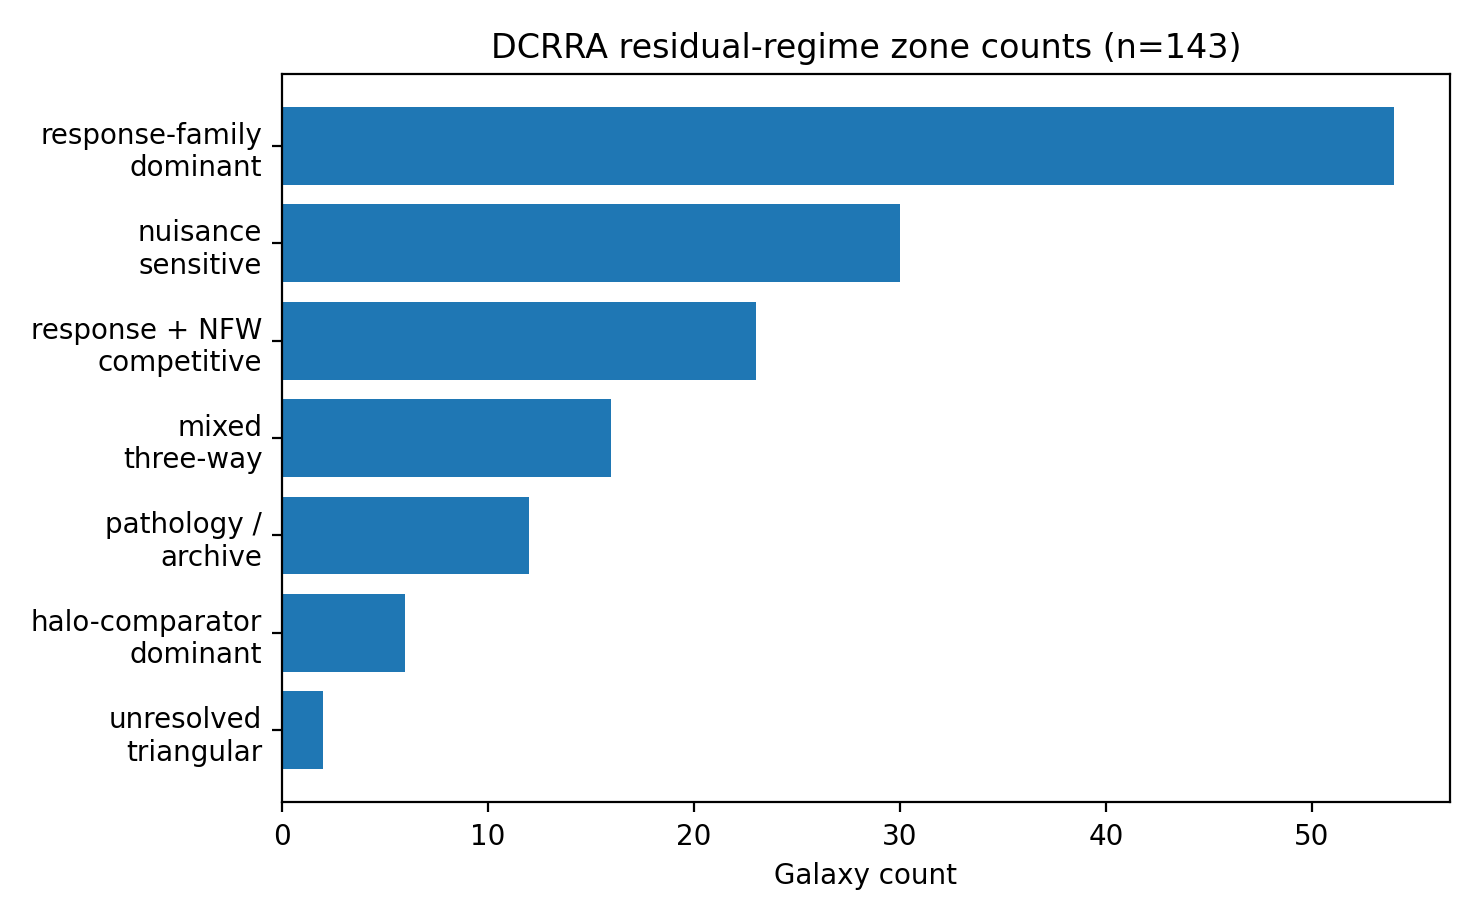
\includegraphics[width=0.84\linewidth]{figs/v301_zone_counts.png}
\caption{Seven-zone DCRRA residual-regime counts. Labels are diagnostic regimes, not physical dark-sector categories.}
\end{figure}

\section{Integrated v3.0.1 phase sequence}
The integrated phase sequence starts from the two parent papers and extends them with new internal audits. Phases 0--3 build the unified residual-response feature table and diagnostic regime-transition adjacency. Phase 4AB uses SPARC public rotmod data for functional residual-shape auditing. Phase 5 expands comparator classes and records overflex-null absorption. Phase 5R tests whether that absorption is sensitive to AIC/AICc/BIC complexity penalties. Phase 6 audits proxy and baryonic-systematics sensitivity. Phase 7 tests frozen holdout robustness. Phase 8 and Phase 8R are intentionally locked as FAIL\_OR\_NULL because the frozen injection-recovery and separability rules do not sufficiently recover or separate synthetic response-like, halo-like, RAR-like, and mixed-like patterns. Phase 9 then converts the limits into a failure-boundary ledger rather than repairing them into a false pass.

\begin{figure}[H]
\centering
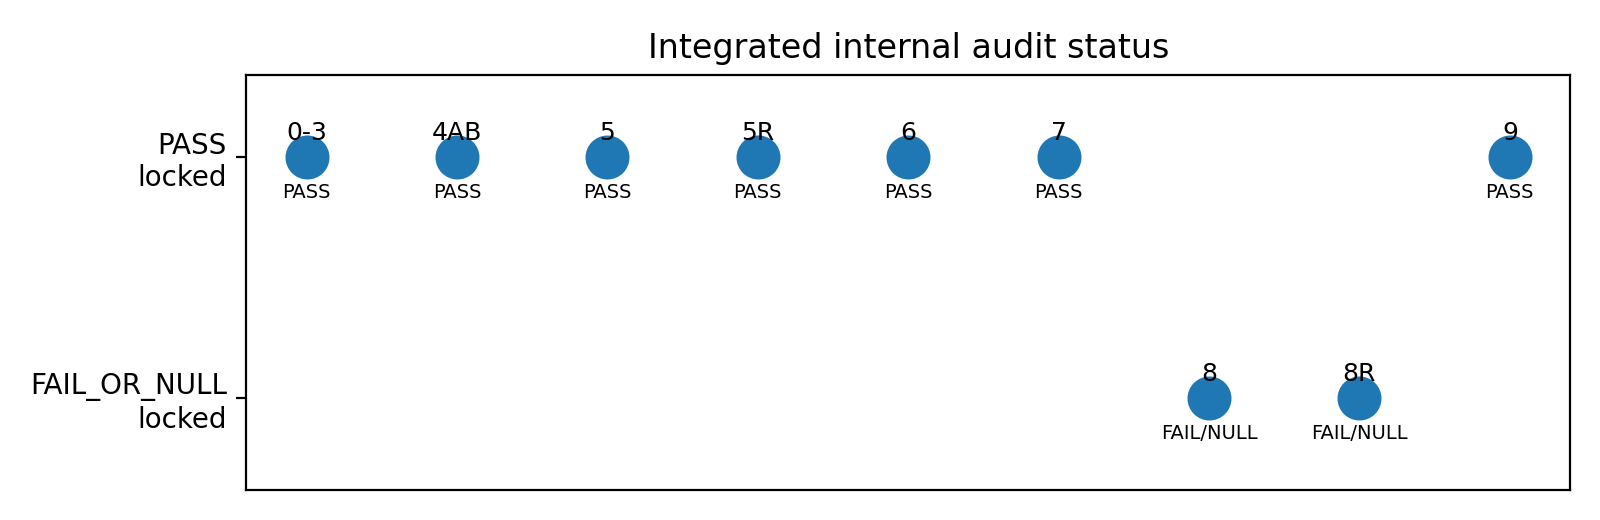
\includegraphics[width=0.88\linewidth]{figs/v301_phase_status.png}
\caption{Integrated internal audit phase status. FAIL\_OR\_NULL phases are retained as first-class evidence.}
\end{figure}

\section{Phase 4AB: functional residual-shape audit}
The SPARC public rotmod files provided 175 galaxy files and matched all 143 galaxies in the integrated feature table. The audit interpolated residual-shape information onto a 40-point common radial grid, producing 5720 shape-grid rows. The first two shape principal components explained 0.827574 and 0.120102 of residual-shape variation, respectively. However, the seven-zone DCRRA map was not reproduced by simple shape clustering; Phase 4B's adjusted Rand index was 0.097191.

This result has a precise interpretation. Residual-shape information is real enough to audit and low-dimensional enough to be meaningful, but it is not sufficient as the whole DCRRA taxonomy. The DCRRA zones should therefore be treated as a multi-layer diagnostic construction involving shape, comparator competitiveness, nuisance sensitivity, pathology handling, and proxy/systematics structure.

\section{Phase 5 and 5R: expanded comparators and overflex-null fairness}
Phase 5 expanded the comparator set and found that an over-flexible polynomial null dominated under the initial AIC criterion, with an overflex winner fraction of 0.860140. Phase 5R then showed that this dominance is sensitive to complexity penalties: the overflex fraction was 0.860140 under AIC, 0.468531 under AICc, and 0.678322 under BIC. In polynomial degree sweeps, the POLY5 fraction was 0.146853 under AICc and 0.160839 under BIC.

The safe interpretation is not that SN-RRF/DCRRA becomes a physical model-selection winner. It is the opposite: comparator wins must not be treated as physical evidence. The expanded comparator audits identify overflex-null absorption and complexity-penalty sensitivity as central failure-boundaries.

\section{Phase 6: proxy and baryonic-systematics sensitivity}
Phase 6 tested 14 proxies and 7 binary outcomes. It found 5 strong proxy split associations. In practical terms, overflex/null behavior and regime behavior are not random with respect to observational and baryonic proxies. The strongest flagged associations included rotation-curve point-count splits, velocity-scale splits, and residual-shape error splits.

This strengthens the diagnostic interpretation while weakening any causal physical over-reading. A regime that tracks observational or baryonic proxies may still be diagnostically useful, but it must not be promoted into a physical dark-sector label without independent domain validation.

\section{Phase 7: frozen holdout robustness}
Phase 7 evaluated 32 holdout conditions excluding the baseline. The stable holdout fraction was 1.000000, with random and zone-leaveout holdout stability also equal to 1.000000. This supports internal robustness under frozen holdout protocols.

However, this is internal SPARC robustness. It does not remove the external-data boundary, and it does not erase the comparator, proxy, or separability cautions. Some restricted subsets change the available zone composition, and the response-family dominant zone carries substantial map weight. Those observations are boundary cautions rather than contradictions.

\section{Phase 8 and 8R: injection-recovery and diagnostic separability limits}
Phase 8 injected synthetic response-family-like, halo-like, RAR-like, nuisance-gradient, pathology/outlier, and mixed response-halo residual patterns. The frozen recovery rule obtained overall recovery 0.566434 and balanced accuracy 0.566434, with only 2/6 guards passed. Low-noise cases were easier, but high-noise recovery dropped to 0.403263. Phase 8R then tested repair/separability variants. Its best full-coverage balanced accuracy remained 0.566434. The physical-like mean recall was 0.432984, while the pathology/nuisance mean recall was 0.833333. The largest off-diagonal confusion was RAR\_LIKE $\rightarrow$ HALO\_LIKE with count 130.

The implication is central to this paper. SN-RRF/DCRRA is more defensible as a residual-regime and failure-boundary diagnostic framework than as a strong physical-category classifier. Pathology and nuisance-like structures are relatively more separable; response-like, halo-like, RAR-like, and mixed-like synthetic patterns remain confusable under the frozen rules.

\section{Phase 9: failure-boundary ledger}
Phase 9 compiles the failure-boundary ledger. This is not an appendix-level afterthought. It is the public-claim control surface for the integrated release. The table below replaces the earlier over-wide table layout with wrapped columns; it is deliberately concise enough to fit the page without right-edge clipping.

\begin{figure}[H]
\centering
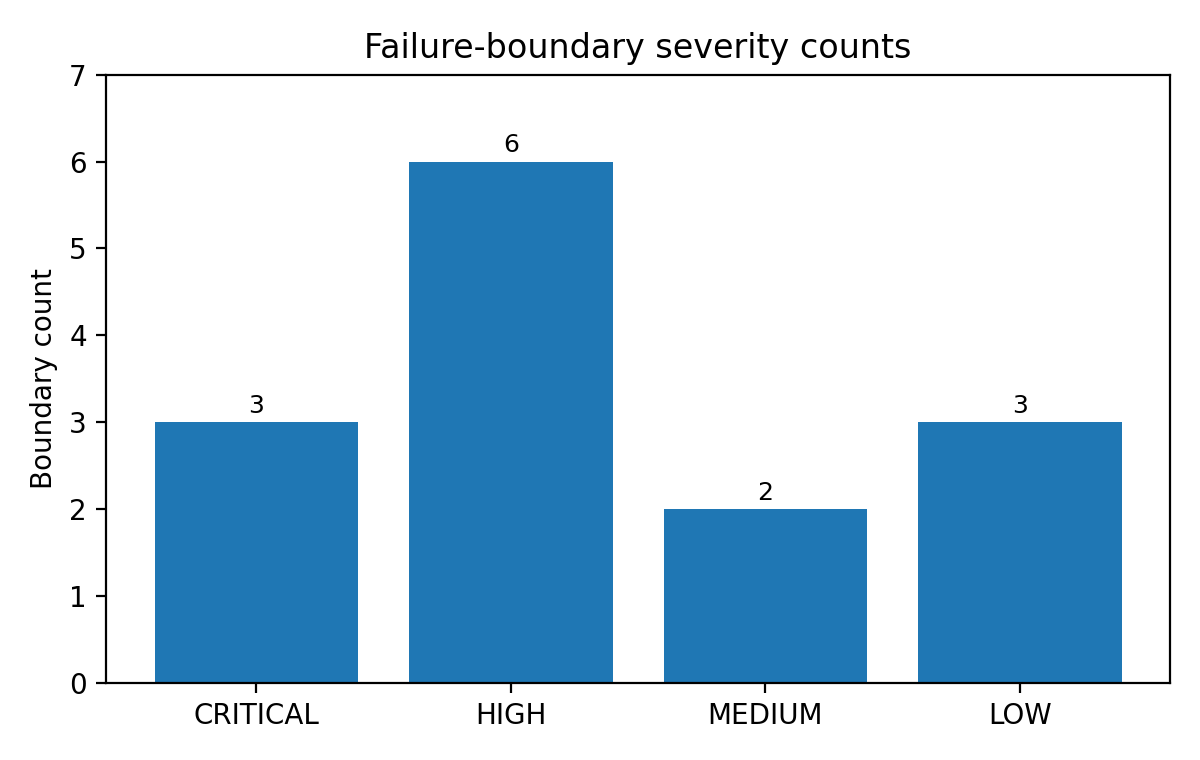
\includegraphics[width=0.64\linewidth]{figs/v301_failure_boundary_severity.png}
\caption{Failure-boundary severity counts in Phase 9. Critical boundaries include external data availability and injection-recovery/separability limitations.}
\end{figure}

{\footnotesize
\setlength{\tabcolsep}{3pt}
\renewcommand{\arraystretch}{1.15}
\begin{longtable}{p{0.09\textwidth}p{0.11\textwidth}p{0.11\textwidth}p{0.14\textwidth}p{0.44\textwidth}}
\caption{Condensed Phase 9 failure-boundary ledger with wrapped public-claim effects.}\\
\toprule
ID & Phase & Severity & Status & Boundary and public-claim effect \\
\midrule
\endfirsthead
\toprule
ID & Phase & Severity & Status & Boundary and public-claim effect \\
\midrule
\endhead
FB-001 & External branch & CRITICAL & HOLD & Full external residual-level validation remains unavailable. Public effect: No external-validation claim. \\
FB-002 & Phase 4AB & MEDIUM & CAUTION & DCRRA zones are not simple residual-shape clusters. Public effect: Do not describe zones as direct shape-template classes. \\
FB-003 & Phase 4AB & LOW & INFORMATIVE & Residual-shape structure is real enough to audit, but not sufficient as taxonomy. Public effect: Permit internal diagnostic shape-language only. \\
FB-004 & Phase 5 & HIGH & CAUTION & Over-flexible null absorbs residual structure in many galaxies. Public effect: No physical model-selection winner claim. \\
FB-005 & Phase 5R & HIGH & CAUTION & Overflex dominance is penalty-sensitive; AIC-only conclusions are unsafe. Public effect: Do not treat AIC comparator dominance as physical evidence. \\
FB-006 & Phase 6 & HIGH & supported boundary & Comparator and regime behavior is associated with observational / baryonic proxies. Public effect: Avoid causal physical classification language. \\
FB-007 & Phase 6 & MEDIUM & CAUTION & A nontrivial subset carries elevated failure-boundary risk. Public effect: Do not hide high-risk cases when reporting population-level structure. \\
FB-008 & Phase 7 & LOW & supported; caution & Frozen holdouts are stable, but boundary cautions remain for restricted subsets and leaveout shifts. Public effect: Internal robustness may be stated only within SPARC protocol. \\
FB-009 & Phase 8 & CRITICAL & FAIL/NULL locked & Synthetic injection-recovery is not sufficiently supported by frozen rules. Public effect: Do not present DCRRA zones as strong classifiers. \\
FB-010 & Phase 8 & HIGH & CAUTION & HALO\_LIKE is weakly recovered under the tested protocol. Public effect: Do not infer stable physical-like template separability. \\
FB-011 & Phase 8 & HIGH & CAUTION & Recovery degrades materially under high-noise injections. Public effect: Avoid general stable-classifier claims. \\
FB-012 & Phase 8R & CRITICAL & FAIL/NULL locked & Separability limitation persists after diagnostic repair audit. Public effect: DCRRA is not a physical-category classifier. \\
FB-013 & Phase 8R & HIGH & CAUTION & Physical-like / comparator-like adjacent types remain confusable. Public effect: Do not use synthetic results to promote response/halo/RAR/mixed labels into physical classes. \\
FB-015 & Phase 0-3 & LOW & carried forward & Earlier boundary notes remain part of v3.0.0 ledger. Public effect: Do not overwrite earlier caveats when integrating new phases. \\
\bottomrule
\end{longtable}
}

\section{External validation status}
Full non-SPARC external residual-level validation remains on HOLD. The missing material is a usable non-SPARC, radius-resolved baryonic component-curve table with sufficient provenance, component definitions, units, and permission for analysis. If such data arrive later, the external branch should restart from manual source-material acceptance rather than from a validation claim.

The SPARC public rotmod audit is valuable, but it is still an internal SPARC audit. It cannot be re-labeled as a non-SPARC external validation.

\section{Integrated synthesis}
The integrated conclusion is stronger than a loose narrative summary and weaker than a physical discovery claim. It is stronger because multiple internal tests support organized diagnostic structure: SN-RRF retains a residual-response-family interpretation; DCRRA preserves a multi-regime residual map; Phase 4AB verifies all 143 galaxies against SPARC rotmod shape data; Phase 6 detects proxy/systematics structure; and Phase 7 supports frozen holdout robustness. It is weaker because Phase 5/5R identify comparator fairness limits, Phase 8/8R fail to support stable synthetic physical-like separability, and non-SPARC external validation remains unavailable.

The consolidated position is therefore: within the internal SPARC diagnostic protocol, SN-RRF/DCRRA provides a structured residual-regime diagnostic framework with explicit comparator, proxy, holdout, injection-recovery, and failure-boundary limitations. It should be used for residual organization, audit prioritization, and failure-boundary mapping, not for physical dark-matter classification or dark-sector replacement claims.

\section{Limitations}
The limitations are first-class results.
\begin{enumerate}
\item All current results are internal to the SPARC diagnostic protocol.
\item Non-SPARC residual-level validation is HOLD.
\item DCRRA zones are not simple residual-shape clusters.
\item Flexible nulls can absorb residual structure.
\item Comparator dominance is complexity-penalty sensitive.
\item Proxy/systematics associations are present.
\item Injection-recovery and diagnostic separability are not sufficiently supported under frozen full-coverage rules.
\item DCRRA zones are not physical-category labels.
\end{enumerate}

\section{Reproducibility}
The repository contains the integrated manuscript sources, phase outputs, runner archives, verification tools, manifest files, claim-boundary documents, release notes, visual orientation files, and the two prior manuscripts as source-lineage materials. Package verification is performed by:
\begin{verbatim}
python tools/verify_manifest_excluding_self.py
python scripts/verify_phase10_package.py
\end{verbatim}
The expected results are manifest verification PASS and integrated package verification PASS.

\section{AI assistance disclosure}
Large language models, including OpenAI ChatGPT, were used as research-assistance tools for theory structuring, verification-protocol organization, code-drafting support, numerical-audit workflow organization, and manuscript editing support. The author remains responsible for the final scientific claims, claim boundaries, interpretation, and manuscript content.

\section{Conclusion}
This manuscript consolidates the SN-RRF parent audit and the DCRRA residual-regime map into an integrated claim-bounded diagnostic framework. The fixed-exponent interpretation does not survive as a universal physical law; the stronger surviving parent object is a scale-normalized monotone-saturating residual-response family. The DCRRA seven-zone map survives as a diagnostic residual-regime taxonomy, not as a physical dark-matter taxonomy. The v3.0.1 integration adds internal shape, comparator, proxy, holdout, injection-recovery, separability, and failure-boundary audits. The final result is a structured diagnostic framework with explicit no-go claims and open external-data requirements.

\begin{thebibliography}{99}
\bibitem{akaike} H. Akaike, A new look at the statistical model identification, \textit{IEEE Transactions on Automatic Control} 19(6), 716--723 (1974). DOI: 10.1109/TAC.1974.1100705.
\bibitem{lelli_sparc} F. Lelli, S. S. McGaugh, and J. M. Schombert, SPARC: Mass Models for 175 Disk Galaxies with Spitzer Photometry and Accurate Rotation Curves, \textit{The Astronomical Journal} 152, 157 (2016). DOI: 10.3847/0004-6256/152/6/157.
\bibitem{rar} S. S. McGaugh, F. Lelli, and J. M. Schombert, Radial Acceleration Relation in Rotationally Supported Galaxies, \textit{Physical Review Letters} 117, 201101 (2016). DOI: 10.1103/PhysRevLett.117.201101.
\bibitem{mond} M. Milgrom, A modification of the Newtonian dynamics as a possible alternative to the hidden mass hypothesis, \textit{The Astrophysical Journal} 270, 365--370 (1983). DOI: 10.1086/161130.
\bibitem{nfw} J. F. Navarro, C. S. Frenk, and S. D. M. White, A Universal Density Profile from Hierarchical Clustering, \textit{The Astrophysical Journal} 490, 493--508 (1997). DOI: 10.1086/304888.
\bibitem{schwarz} G. Schwarz, Estimating the Dimension of a Model, \textit{The Annals of Statistics} 6(2), 461--464 (1978). DOI: 10.1214/aos/1176344136.
\bibitem{hurvich_tsai} C. M. Hurvich and C.-L. Tsai, Regression and time series model selection in small samples, \textit{Biometrika} 76(2), 297--307 (1989). DOI: 10.1093/biomet/76.2.297.
\bibitem{yoshimura_snrrf} K. Yoshimura, \textit{Claim-Bounded Diagnostics for SPARC Galaxy Rotation-Curve Residuals: Scale-Normalized Residual-Response Family Tests and Null-Control Audits}, independent manuscript and repository package (2026). Repository archive DOI: 10.5281/zenodo.20224479.
\bibitem{yoshimura_dcrra} K. Yoshimura, \textit{Claim-Bounded Diagnostics for Dark-Component-like SPARC Rotation-Curve Residuals: Residual-Regime Mapping, Comparator Audits, and Null-Control Checks}, independent manuscript and repository package (2026). Repository archive history: 10.5281/zenodo.20233908.
\end{thebibliography}

\end{document}
